%	Name			:: 	sthlm Beamer Theme  HEAVILY based on the hsrmbeamer theme (Benjamin Weiss)
%	Author			:: 	Mark Hendry Olson (mark@hendryolson.com)
%	Created			::	2013-07-31
%	Updated	    	::	[[April]] 04, 2017 at 16:26:39
%	Version			:: 	2.0.2
%	Email			:: 	hendryolson@gmail.com
%	Website			:: 	http://markolson.se
%	Twitter			:: 	markolsonse
%	Instagram		:: 	markolsonse
%
%	License			:: 	This file may be distributed and/or modified under the
%					GNU Public License.
%
%	Description		::	This presentation is a demonstration of the sthlm beamer
%					theme, which is HEAVILY based on the HSRM beamer theme created by Benjamin Weiss
%					(benjamin.weiss@student.hs-rm.de), which can be found on GitHub
%					<https://github.com/hsrmbeamertheme/hsrmbeamertheme>.  It also borrows heavily
%					from the work of Matthias Vogelgesang, (https://bloerg.net) and his Metropolis Mtheme,
%					<https://github.com/matze/mtheme>.
%
%	Theme			::	newPxFont
%	Options			::	progressbar
%					::	sectionpages
%					::	numfooter
%					::	fullfooter
%					::	dovaligncolumns
%					::	protectframetitle
%					::	greybg
%					::	cblock
%					::	minimal


%-=-=-=-=-=-=-=-=-=-=-=-=-=-=-=-=-=-=-=-=-=-=-=-=
%
%        LOADING DOCUMENT
%
%-=-=-=-=-=-=-=-=-=-=-=-=-=-=-=-=-=-=-=-=-=-=-=-=

\documentclass[newPxFont,numfooter,sectionpages]{beamer}
\usepackage[utf8]{inputenc}
\usetheme{sthlm}
\usepackage{pgfplots}
\pgfplotsset{compat=1.14}
\usepackage{cancel}
\usepackage{xcolor}

%-=-=-=-=-=-=-=-=-=-=-=-=-=-=-=-=-=-=-=-=-=-=-=-=
%
%	PRESENTATION INFORMATION
%
%-=-=-=-=-=-=-=-=-=-=-=-=-=-=-=-=-=-=-=-=-=-=-=-=



\title{\Large{{Entwicklung und Implementierung eines\\ userinput- und scriptgesteuerten, betriebssystemunabhängigen Networking-Interfaces unter Zuhilfenahme eines eigenständig entwickelten Protokolls}}}

\date{22. September 2017, Erfurt}
\author{Leonard Petereit, Jan Sommerfeld, Benedikt Schäfer}
\institute{\footnotesize{Spezialschulteil des Albert-Schweitzer Gymnasiums Erfurt}}

\hypersetup{
pdfauthor = {Mark H. Olson: hendryolson@gmail.com},
pdfsubject = {Beamer},
pdfkeywords = {Beamer theme, sthlm},
pdfmoddate= {D:\pdfdate},
pdfcreator = {test}
}

\begin{document}

\begin{frame}
\vspace*{8mm}
\centering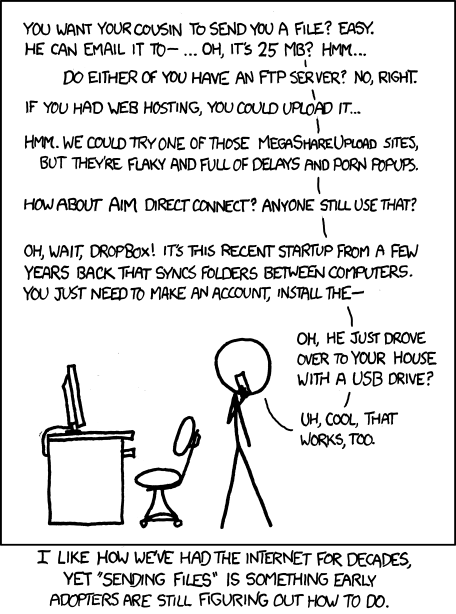
\includegraphics[scale=0.34]{in}
\end{frame}

%-=-=-=-=-=-=-=-=-=-=-=-=-=-=-=-=-=-=-=-=-=-=-=-=
%
%	TITLE PAGE
%
%-=-=-=-=-=-=-=-=-=-=-=-=-=-=-=-=-=-=-=-=-=-=-=-=

\maketitle

%-=-=-=-=-=-=-=-=-=-=-=-=-=-=-=-=-=-=-=-=-=-=-=-=
%	FRAME: Theme Package Requirements
%-=-=-=-=-=-=-=-=-=-=-=-=-=-=-=-=-=-=-=-=-=-=-=-=
%\begingroup
%\setbeamercolor{frametitle}{bg=\cnRed}
%\setbeamercolor{normal text}{fg=\cnDarkGrey,bg=\cnLightRed}
%\begin{frame}{Please use Metropolis Theme Instead}
%
%Thank you for wanting to use sthlm.
%
%\vspace{1em}
%
%However, \textbf{you really should consider} using the Metropolis (mTheme) theme developed by Matthias Vogelgesang and the LaTeX community instead as it is very well maintained and documented.
%
%\begin{center}
%	\cBlue{\url{https://goo.gl/r683yn}}
%\end{center}
%\end{frame}
%\endgroup
%

%-=-=-=-=-=-=-=-=-=-=-=-=-=-=-=-=-=-=-=-=-=-=-=-=
%
%	TABLE OF CONTENTS: OVERVIEW
%
%-=-=-=-=-=-=-=-=-=-=-=-=-=-=-=-=-=-=-=-=-=-=-=-=

\section*{Overview}
\begin{frame}{Overview}
% For longer presentations use hideallsubsections option
\tableofcontents[hideallsubsections]
\end{frame}

%-=-=-=-=-=-=-=-=-=-=-=-=-=-=-=-=-=-=-=-=-=-=-=-=
%
%	TABLE OF CONTENTS: OVERVIEW
%
%-=-=-=-=-=-=-=-=-=-=-=-=-=-=-=-=-=-=-=-=-=-=-=-=
\section{Differenzierung des Themas und Zielstellungen}
\begin{frame}
\frametitle{Differenzierung des Themas und Zielstellungen}
\begin{itemize}
\item Wissenszuwachs
\item Dateitransfer 
\item Entwicklung eines Netzwerkinterfaces
\item Entwicklung eines Protokolls
\item Dynamische Verarbeitung von User-Eingaben
\item Implementierung


\end{itemize}
\end{frame}

\section{Benötigte Methoden zum Erreichen der Zielstellungen}
\begin{frame}
\frametitle{Benötigte Methoden zum Erreichen der Zielstellungen}
\begin{itemize}


\item{Literaturstudium}
\item{Protokoll-Design}
\item{Syntax-Design}
\item{Evaluierung}
\item Programmierung
\end{itemize}

\end{frame}

\section{Geplante zeitliche Orientierung}
\begin{frame}
\frametitle{Geplante zeitliche Orientierung}
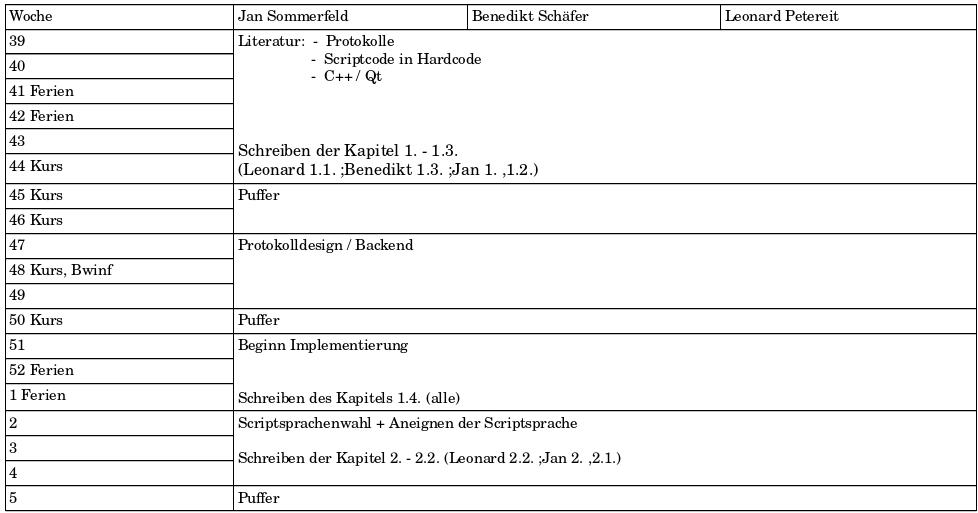
\includegraphics[scale=0.31]{z}
\end{frame}
\begin{frame}
\frametitle{Geplante zeitliche Orientierung}
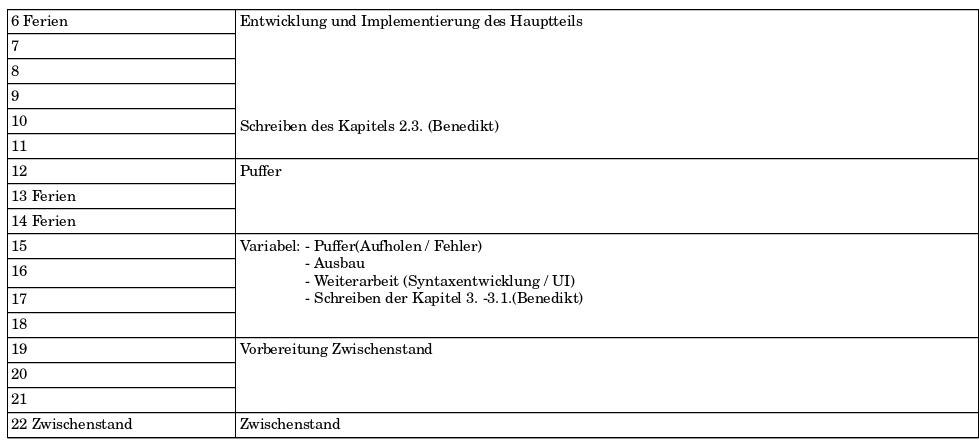
\includegraphics[scale=0.31]{z1}
\end{frame}

\begin{frame}
\frametitle{Quellen}
\begin{itemize}
\item{https://xkcd.com/949/}
\end{itemize}

\end{frame}
\end{document}